\section{Base system}
In this section, you can find a brief explanation of the different items. When you execute the application, you see two windows:
\begin{enumerate}
\item One of them is the Gateway of the smart home:
\begin{center}
	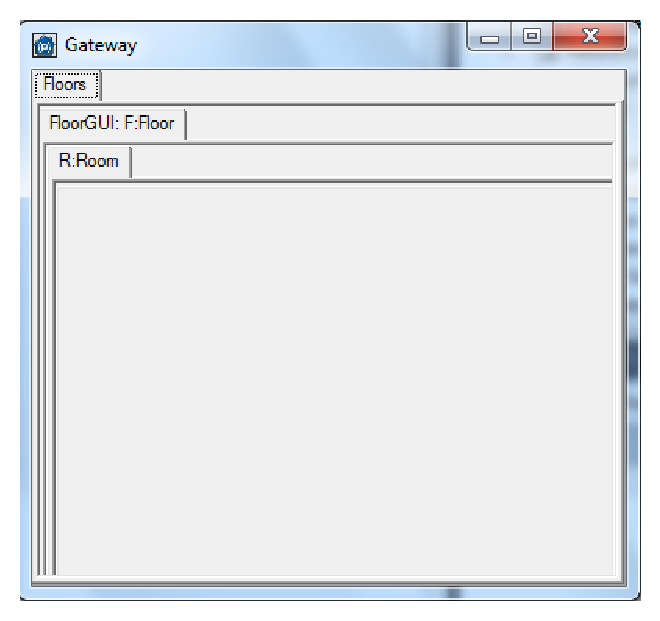
\includegraphics[width=.55\linewidth]{images/gateway.eps}
	\\
	\vspace{1cm}
\end{center}
In this window, you could change the values of the actuators. Each characteristic has a global tab and a tab in the rooms that it belongs.
\item Simulator:
\begin{center}
	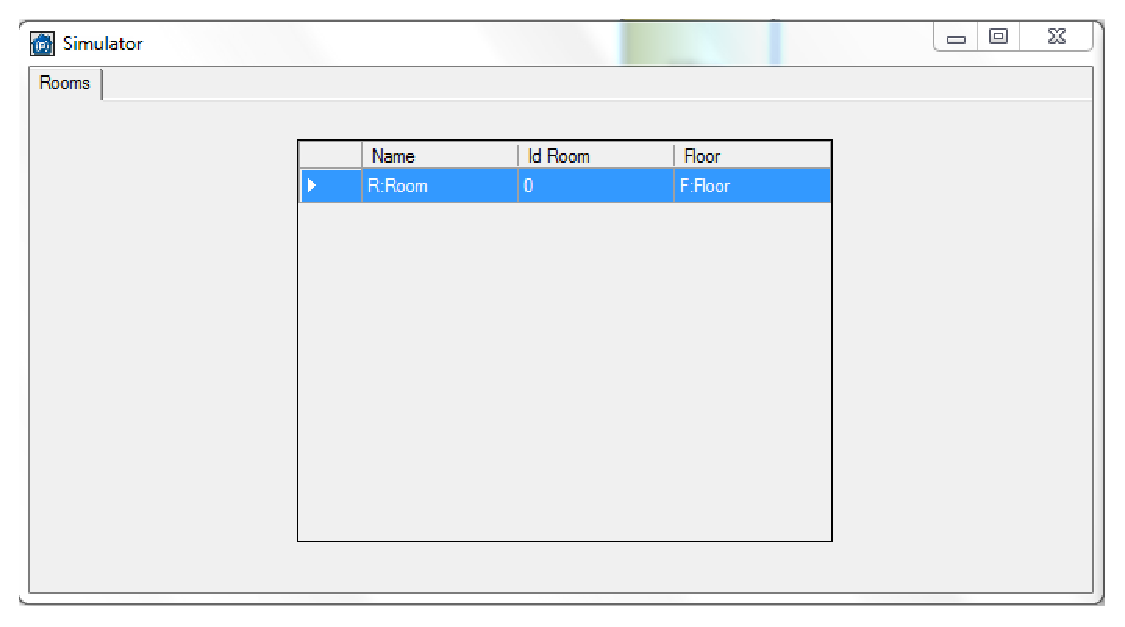
\includegraphics[width=.68\linewidth]{images/simulator.eps}
	\\
\vspace{1cm}
\end{center}
This window is only for simulator purposes. For each characteristic, you could find a tab where you can see the status of the items and change the values of elements like thermometers, time system...
\end{enumerate}